\documentclass[12pt]{article}

% Basic stuff
\usepackage{fullpage}
\usepackage{graphicx}
\usepackage[parfill]{parskip}
\usepackage[utf8]{inputenc}

% Skip one line between paragraphs
\parskip1em
 
% Standard things to include for math   
\usepackage{amsmath,amssymb,amsfonts,amsthm}

% Other stuff
\usepackage{hyperref}
\usepackage{datetime} \usdate
\usepackage{enumitem}
\usepackage{changepage}


% Some of Ebrahim's definitions
\newcommand{\note}[1]{[#1]}
\newcommand{\done}{\\\hspace*{0pt}\hfill$\blacksquare$}
\def\N{\mathbb{N}}
\def\R{\mathbb{R}}
\def\Q{\mathbb{Q}}
\def\Z{\mathbb{Z}}
\def\e{\varepsilon}
\def\d{\delta}
\newcommand{\seq}[1]{\left(#1\right)_{n\in\N}}
\newcommand{\settext}[2]{\left\{ #1\ |\ \text{#2} \right\}}
\renewcommand{\emptyset}{\{\hspace{-2pt}\}}
\newcommand{\powerset}[1]{\mathcal{P}(#1)}
\newcommand{\dom}[1]{\operatorname{dom}(#1)}
\newcommand{\ran}[1]{\operatorname{ran}(#1)}
\newcommand{\rev}[1]{(#1)^{\dashv}}
\newcommand{\injrightarrow}{\xrightarrow{\text{inj}}}
\newcommand{\surjrightarrow}{\xrightarrow{\text{surj}}}
\newcommand{\bijrightarrow}{\xrightarrow{\text{bij}}}
\newcommand{\AND}{\wedge}
\newcommand{\OR}{\vee}
\newcommand{\ex}[1]{\textbf{Exercise:}\begin{adjustwidth}{2em}{}#1\end{adjustwidth}}



\begin{document}

\begin{center} {\Large \scshape Mathematical Proofs and Mathematical Writing}
\end{center}
(compiled on \today\ at\ \currenttime)
\hfill

\tableofcontents

\section{Introduction}

\note{what to put here:
this course is about both set theory and writing.
set theory is axiomatic. describe what i mean by that, why we would do that, and the historical relevance of it.
why rigor anyway?
logic can also be done this way, but we will not.
we will follow a more intuitive and informal writing-focused approach for logic,
saving our rigor-enegery for set theory.
perhaps include a discussion levels of rigor and formality, with one level relegating the rigor to other levels.
mention the importance of writing and the roughness of this transition for many people.
mention the value of forgetting what you knew before, but not really forgetting it all.}

\note{Write the general intro later, maybe last.}



\section{Mathematical Language}
\label{sec:logic}

This section will develop mathematical logic and show you how logical arguments factor into writing.
We do not yet have anything to argue \emph{about}, so our ``proofs'' will be about nothing in particular.
Section \ref{sec:sets} will later give some mathematical objects to talk about, and we will then put
content into the empty skeleton arguments of this section.

\subsection{Parts of Speech}

In a language, a \emph{part of speech} is a collection of words that share grammatical properties.
For example here are some common English parts of speech: pronouns, nouns, verbs, adjectives, and adverbs.
Different languages can have different parts of speech that are useful for describing their grammar.
To build up the grammar of a language, one can specify how parts of speech fit together to form larger
\emph{constituents}, such as noun phrases and clauses. One can further describe how
constituents fit together to form even more complex constituents, eventually grammatical sentences.

Mathematics is a language, and so it makes sense to build up its grammar (its \emph{syntax}) using this same strategy.
Instead of pronouns, nouns, verbs, noun phrases, sentences, and so on, there are just four constitutuents in
mathematics. Two are basic parts of speech and two are more complex constituents:
\begin{itemize}
\item \emph{Variables} are a basic part of speech.
\item \emph{Constants} are a basic part of speech.
\item \emph{Terms} can be built out of variables, constants, other terms, and propositions.
\item \emph{Propositions} can be built out of variables, constants, terms, and other propositions.
\end{itemize}

Let's go through each of these in detail.

\def\sp{\hspace{1em}}
\paragraph{Variables}
Variables serve as placeholders, waiting to be replaced by other symbols.
They are most like pronouns in English.
For example the pronoun ``it'' is a placeholder referring to something in a discussion, but what it refers to depends on the context of the discussion.
Variables are like that.
Here are some variables:
\begin{center}
$a$ \sp $b$ \sp $A$ \sp $f$ \sp $q$ \sp $x$\sp $\alpha$\sp $\beta$
\end{center}
Variables are copies of letters coming from an alphabet (usually Latin or Greek) and written in ink/chalk/pixels.



\def\sp{\hspace{1em}}
\paragraph{Constants}
Constants are used as fixed names for specific mathematical objects.
They are most like \emph{proper} nouns in English.
Here are some constants:
\begin{center}
$0$ \sp $1$ \sp $2$ \sp $3$ \sp $4$ \sp $5$ \sp $6$ \sp $7$ \sp $8$ \sp $9$ \sp $\N$ \sp $\R$ \sp $\emptyset$
\end{center}
The difference between constants and variables is that constants are not meant to be substituted for.
The constant ``$2$'' refers to a specific thing, rather than being a placeholder for something.


Note that we are mainly talking about elements of \emph{language}, and not about what those elements \emph{refer} to.
Germany is not a noun, it's a country. ``Germany'' is, however, a noun.
Similarly, we can say that $2$ is not a constant, but rather ``$2$'' is.
And $x$ is not a variable, but rather ``$x$'' is.
Quotation marks help us make the distinction between a symbol and what the symbol refers to.




\def\sp{\hspace{1em}}
\paragraph{Terms}
Terms are strings of marks (expressions) that refer to \emph{mathematical objects}.
Since variables and constants refer to mathematical objects, they are special cases of terms.
But you can also have more complicated terms that are built out of simpler ones.
Terms are most like \emph{noun phrases} in English.
For example the phrase ``the cup that you drank from'' is a noun phrase;
it doesn't make any assertion but rather it just refers to a \emph{thing}.
Here are some terms:
\begin{itemize}[label=\sp]
\item $x$
\item $7$
\item $\{2,3,a,7\}$
\item $f(x)$
\item $\{(z,w)\} \circ g$
\item $S\times Q$
\item the square of the seventh prime number
\item a triangle
\item twelve dimensional euclidean space
\item the collection of even integers
\item $\settext{n}{$n\in\Z$ and $n$ is even}$
\item $\settext{n}{$(n\in\Z)\AND (\exists k\,|\,(k\in\Z)\AND(2k=n))$}$
\end{itemize}
The last three terms actually refer to the same mathematical object; this will soon become clear
when we get into \emph{how} the symbols refer to objects (semantics). For now we are only looking at
\emph{which} strings of symbols \emph{can} refer to objects (syntax).
You can see that some terms are more ``symbolic,'' while others are more ``Englishy.''
The formal language of mathematics is purely symbolic,
but we almost never use the language in its purest form.
Typically, we communicate by some combination of English and mathematics.


\def\sp{\hspace{1em}}
\paragraph{Propositions}
Propositions are strings of marks (expressions) that \emph{make assertions}.
They are most like \emph{sentences} in English (sentences in the indicative mood).
Propositions can be true or false. 
Here are some propositions:
\begin{itemize}[label=\sp]
\item $x\in S$.
\item $5\notin x$.
\item $0=2$.
\item $(x\neq y) \AND (x\neq z) \AND (y\neq z)$.
\item $x$, $y$, and $z$ are distinct.
\item Either $A\subseteq P$ or $x\in S$, but not both.
\item $f:X\rightarrow Y$.
\item If $x\in S$, then we either have $x\notin W$ or we have $x\in\Z$.
\item $\neg(X\times Y \subseteq Z)$.
\item Every integer is even.
\item $(\forall n \, | \, (n\in\Z)\Rightarrow (\exists k\,|\,(k\in\Z)\AND(2k=n)))$.
\end{itemize}
The last two propositions are actually saying the same thing, as we will see when we get into semantics.
Again, you can see that some propositions are more ``symbolic,'' while others are more ``Englishy.''
Typically, we make mathematical assertions by using some combination of English and mathematics.
The English that we use is a crude, but human-friendly, stand-in for formal mathematical statements.



\ex{
Determine whether each of the following is a term or a proposition.
\begin{enumerate}
\item $n$
\item $1+1=0$
\item $n$ is an odd integer
\item an odd integer
\item $f$ is a function with domain $S$
\item $1+(2+3)$
\item the empty set
\item the sum of two vectors is another vector
\item the zero vector
\item the evenness of $2$ % this one is a trick, it's neither unless you are doing metamathematics
\end{enumerate}
}

\subsection{Theorems and Proofs}

Mathematics is ultimately about propositions.
Propositions \emph{say} things, sometimes true things and sometimes false things.
We want to know: Which propositions are true? What does ``true'' even mean?
We will not exactly define ``true,'' but we will define ``provable,''
and provability will be our notion of truth.

The rules of logic allow us to make deductions and \emph{prove} new propositions
from already proven propositions.
Those already proven propositions themselves had to be proven via a sequence of logical deductions
that was applied to other previously proven propositions.
And so on...
but where does it all start?

\paragraph{Axioms}
Some propositions are declared to be \emph{axioms},
which makes them serve as starting points in our mathematical system.
The next paragraph will clarify this.

\paragraph{Proofs}
A \emph{proof} is a sequence of propositions such that each proposition is either
(1) an axiom, 
(2) an already proven proposition,
or, (3) the result of applying the rules of logic to \emph{previous} propositions in the sequence.
A proposition that appears in a proof is said to be \emph{proven}.


\paragraph{Theorems}
A \emph{theorem} is a proposition which is asserted to have a proof.

\subsubsection{Example of a Formal Proof}


\def\ES{\settext{x}{$x\neq x$}}

Below is an example of a proof of the proposition ``$(\forall x\,|\,x\notin\ES)$''.
\begin{adjustwidth}{1cm}{}
$(x\in\ES)\Longrightarrow (x\neq x)$\\ 
$(x=x)\Longrightarrow (x\notin \ES)$\\
$x=x$\\
$x\notin\ES$\\
$(\forall x\,|\,x\notin\ES)$
\end{adjustwidth}
Here I don't want you to worry about interpreting what the propositions are trying to \emph{say};
I just want to demonstrate how a theorem arises as a result of applying the rules of logic
to various axioms. What you see above is a sequence of five propositions, ending with the
one I claimed to be proving, namely ``$(\forall x\,|\,x\notin\ES)$''.
To really be convinced that we are looking at a proof, we would need a \emph{justification}
for each of the five propositions-- for each proposition we need to either point out that it is
an axiom, or we need to verify that it follows logically from the previous propositions.
In this example, two of the propositions are axioms, and the other three are logical deductions;
here is a schematic depiction of these relationships:
\begin{center}
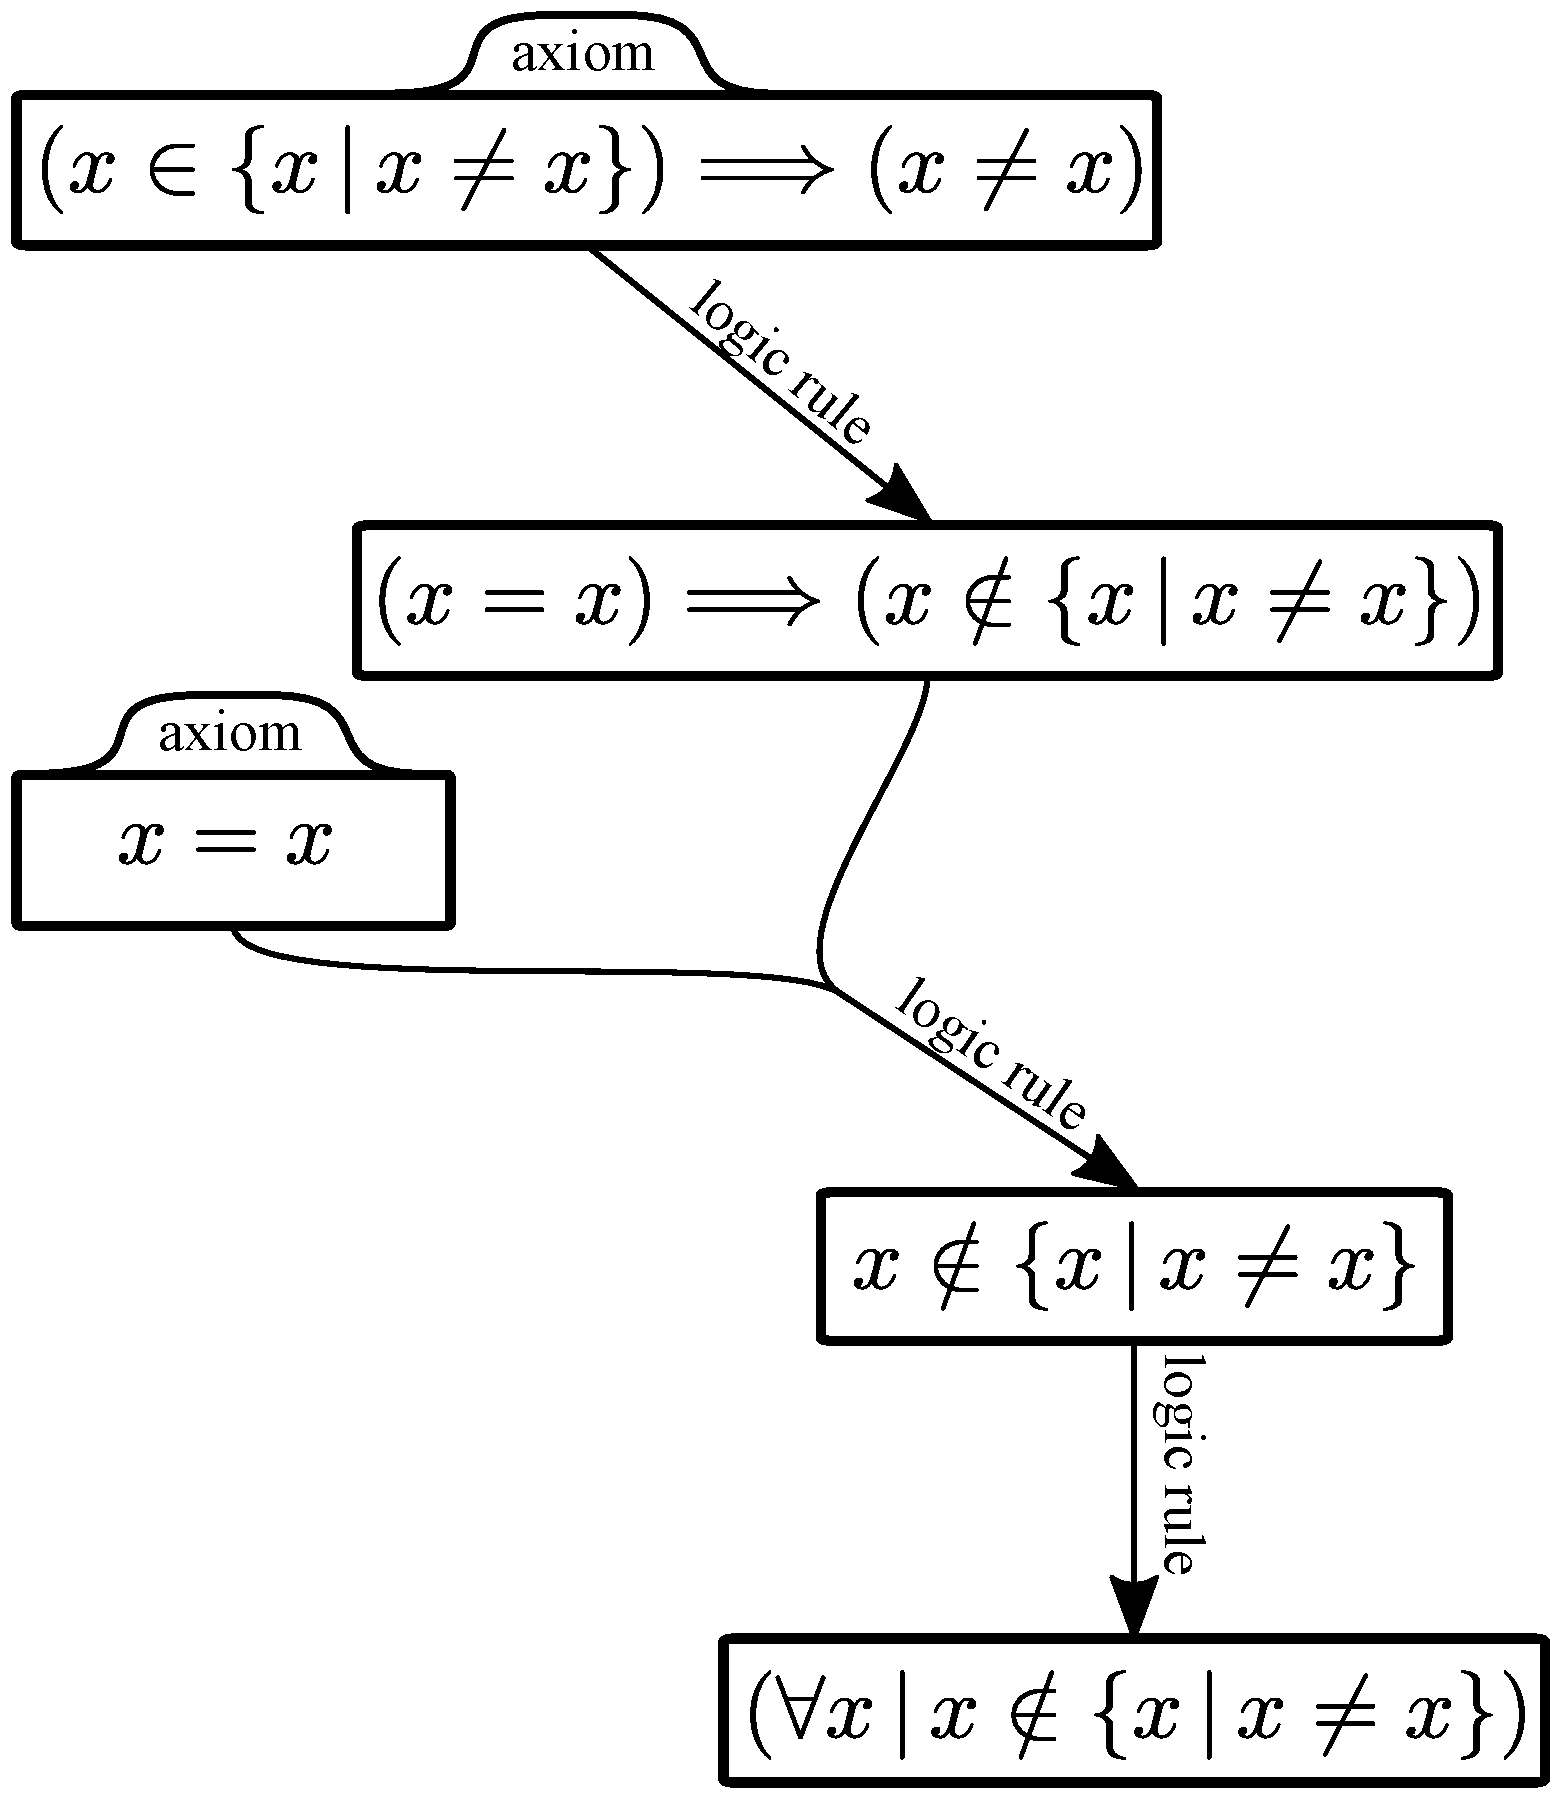
\includegraphics[scale=0.25]{proofFlow.pdf}
\end{center}
Again, don't worry yet about understanding why this works.
What I want you to take away from this is the general structure:
we have axioms serving as starting propositions, and we use logic to ``flow'' out from
the starting points and prove other propositions.

Given a bunch of axioms to start with, what theorems can we deduce?
To answer this question is to do math.

\paragraph{Remark about Axioms}
Axioms often serve to \emph{give meaning} to symbols.
For example, the axiom $x=x$ (along with some other axioms related to equality)
gives meaning to the symbol ``$=$''.
Without the axiom, we would still be able to form propositions like $a=b$ but we would never be able to
prove anything about them.
Suppose you ``disagree'' with the axiom $x=x$ and instead use some other propositions related to ``$=$'' as axioms.
That's perfectly fine-- you would just be giving a different meaning to the symbol ``$=$'' and it would serve a different purpose in your language.

\paragraph{Math is for Humans}
The five-line proof given above is a \emph{formal proof}-- it is written in pure mathematical language
with absolutely no English.
This is great if you want absolute rigor, but
it is not friendly to read if you are not a computer.
The main purpose of a mathematical proof is for it to convince a human that a theorem is true.
But formal proofs make for really inefficient communication between humans.
Thus we are faced with a trade-off: 
we can sacrifice some rigor to gain efficiency of communication.

\emph{Informal proofs} use a mixture of English and mathematics to make arguments.
For an example, look ahead a few paragraphs for an informal version of the five-line proof above.

We need to find a good balance between rigor and efficient communication.
Finding that balance is one of the great challenges when you first learn how to write proofs.
If we sacrifice too much rigor in an argument, then we can lose confidence in its correctness.
Or worse, we can start to prove false things!
When developing a new mathematical theory, it's generally good to err on the side of being more rigorous.
Then, as the theory develops and common patterns of arguments become routine,
one can slowly relax the rigor in favor of efficiency.

Now you can see what this course is all about.
While it is partly giving you some specific mathematical content like set theory,
this course is mainly about how to communicate proofs in that balanced way-- rigorous, yet informal and efficient.

Here is an informal version of the five-line proof from above.

\paragraph{Theorem} The set $\ES$ has no elements.

\textit{Proof:}
If $\ES$ did have an element, say $x$, then we would have $x\neq x$.
But in fact it is an axiom that $x=x$. Thus $\ES$ cannot have any elements.
\done

The arguments are essesntially the same ones that appeared in the five-line formal proof.
But, compared to the formal proof, it's much easier to process the arguments (though I'm still not expecting you to do so just yet).

\newpage 
\def\s{0.25}
\newcommand{\rb}[1]{\raisebox{-0.2em}{#1}}
\ex{
In this exercise we will work with a made-up deductive language which works as follows:
\begin{itemize}
\item Propositions are the only part of speech. The propositions are $3\times 3$ grids in which each square is either blank or contains a dot. Here are three random example propositions:
\begin{center}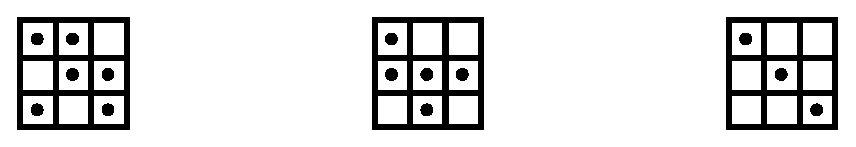
\includegraphics[scale=\s]{gridgame1.pdf}\end{center}
\item There are two logical rules in this language.
The first rule is that if a particular proposition holds, then
its clockwise rotation by ninety degrees follows. So if 
\rb{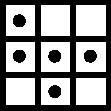
\includegraphics[scale=\s]{gridgame2.pdf}}
holds, then you can deduce that
\rb{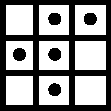
\includegraphics[scale=\s]{gridgame3.pdf}}.
The second rule is that if two propositions $\Phi$ and $\Psi$ hold, then you can deduce a third proposition
which contains a dot in any square that has a dot in either $\Phi$ or $\Psi$, but not both.
So for example if you have the two propositions
\rb{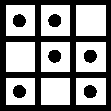
\includegraphics[scale=\s]{gridgame6.pdf}}
and
\rb{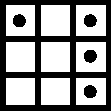
\includegraphics[scale=\s]{gridgame7.pdf}},
then you can deduce from them that
\rb{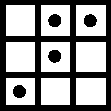
\includegraphics[scale=\s]{gridgame5.pdf}}.
\item There are only two axioms in this language, and they are as follows:
\begin{center}
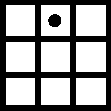
\includegraphics[scale=\s]{gridgame8.pdf}
\hspace{2em}
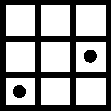
\includegraphics[scale=\s]{gridgame9.pdf}
\end{center}
\end{itemize}
As a demonstration of this deductive language, here is a proof that 
\rb{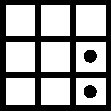
\includegraphics[scale=\s]{gridgame11.pdf}}\ :
\begin{center}
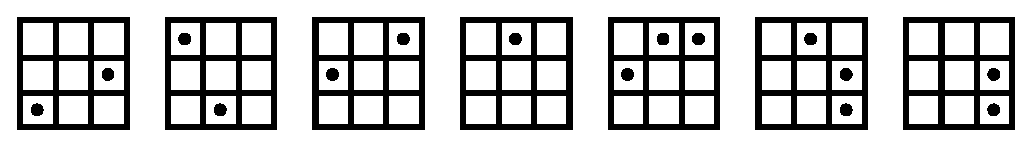
\includegraphics[scale=\s]{gridgame10.pdf}
\end{center}
Can you see how this proof is correct?
These annotations may help:
\begin{center}
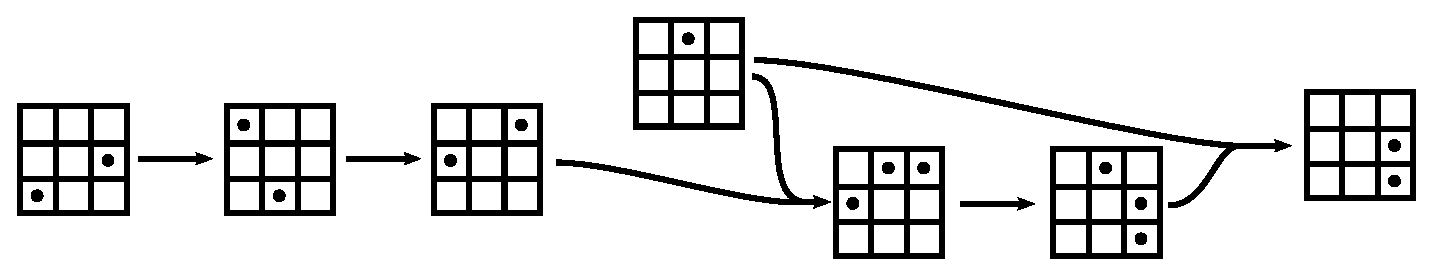
\includegraphics[scale=\s]{gridgame12.pdf}
\end{center}
Now...
\begin{enumerate}
\item
How many propositions are there in this language?
How many propositions do you think there are in mathematics?
How many sentences are there in English?
\item
Give a completely formal proof that 
\rb{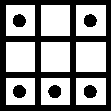
\includegraphics[scale=\s]{gridgame0.pdf}}.
To help out your reader, annotate the proof with arrows like in the example above.
\item (Open-ended) Can you think of a way to write an \emph{informal} version of your proof?
It would be an English description of your proof that does not explain every detail but still captures the essence of your formal proof.
%One way to think of an informal proof is: it somehow gives the reader \emph{instructions} for how to come up with the formal proof.
\item (Irrelevant but fun) Can you figure out how many propositions in this language are provable and how many are not?
\end{enumerate}
}



\subsection{Logic and Writing Mathematical Arguments}

% the rest of the course is logic and set theory with the goal of being able to write balanced informal proofs
% now that you know what a deduction system is, we will go through some of the rules of mathematical logic and look at the form they take in our written proofs.

% run through the rules and some useful derived rules of logic
% the focus is not formal derivation, but rather to make the rules intuitive and to examine how they influence *writing*
% where truth tables can help make rules intuitive, bring them in. otherwise truth tables are not a main focus


% a comment (maybe put this earlier) on how repetitiveness is okay for now, and better to fix it later. perhaps sian comments on how fix


\section{Set Theory} % and still writing though...
\label{sec:sets}


% develop set theory along the lines of jacoby notes

% some milestones to reach: relations, functions, induction, recursion, natural numbers

% appendix: put some sample well written proofs and badly written proofs




\end{document}



